\documentclass[xcolor=table,xetex,mathserif,serif]{beamer}
% % Hyperlinks.
\usepackage{hyperref}
% \hypersetup{
%     colorlinks=true,
%     linkcolor=blue,
%     filecolor=magenta,      
%     urlcolor=blue,
% }

% Language settings.
\usepackage{polyglossia}
\setdefaultlanguage[babelshorthands=true]{russian}

% Setting outer theme.
\useoutertheme{infolines}

% Setting font.
\usepackage{fontspec}
\setmainfont{FreeSans}
\newfontfamily{\russianfonttt}{FreeSans}

% Code highlighting.
\usepackage[outputdir=temp]{minted}
\usepackage{xcolor}

% Images.
\usepackage{graphicx}
\usepackage{animate}

\title{CV parse}
\author[трое в .KE]{трое в .KE}
\date{20.09.2020}

\begin{document}

\begin{frame}
	\titlepage{}
\end{frame}


\begin{frame}
	\frametitle{Постановка задачи}

	\begin{itemize}
		\item 2 таблицы
		      \begin{itemize}
			      \item резюме
			      \item вакансии
		      \end{itemize}
		\item 3 модели
		      \begin{itemize}
			      \item офицант
			      \item кладовщик
			      \item водитель погрузчика
		      \end{itemize}
		\item выделить формализованную модель
	\end{itemize}
\end{frame}


\begin{frame}
	\frametitle{Подход к решению}

	\begin{itemize}
		\item Нет размеченных данных
            \begin{itemize}
                \item сложно применять методы глубокого обучения и сложно интерпретировать результаты
            \end{itemize}
		\item Данные большие и неструктурированные
		      \begin{itemize}
			      \item разбить вопросы на общие и специфические
			      \item в ответах на общие вопросы содержатся ответы на специфические
			      \item данные не теряются при разбиении
		      \end{itemize}
	\end{itemize}
\end{frame}


\begin{frame}
	\frametitle{Предложенная модель}

	\begin{table}[]
		\resizebox{0.6\columnwidth}{!}{
			\begin{tabular}{|l|l|l|}
				\hline
				\multicolumn{3}{|c|}{\textbf{Кладовщик (дано)}}          \\ \hline
				\rowcolor[HTML]{DAE8FC}
				Переменная & Описание                   & Тип данных     \\ \hline
				q1         & Желаемая должность         & string         \\ \hline
				\rowcolor[HTML]{EFEFEF}
				q2         & \begin{tabular}[c]{@{}l@{}}У вас есть опыт \\ работы кладовщиком?\end{tabular}  & boolean        \\ \hline
				q2d        & \begin{tabular}[c]{@{}l@{}}У вас есть опыт \\ работы кладовщиком?\end{tabular}  & string         \\ \hline
				\rowcolor[HTML]{EFEFEF}
				q3         & \begin{tabular}[c]{@{}l@{}}Укажите Ваш стаж \\ работы кладовщиком\end{tabular}  & integer        \\ \hline
				q4         & Отрасль                    & string (array) \\ \hline
				\rowcolor[HTML]{EFEFEF}
				q5         & Названия компаний          & string (array) \\ \hline
				q6         & \begin{tabular}[c]{@{}l@{}}С какой системой хранения \\ Вы имели опыт работы?\end{tabular}  & string (array) \\ \hline
				\rowcolor[HTML]{EFEFEF}
				q7         & Опыт работы с программами  & string (array) \\ \hline
				q8         & Опыт с инструментарием     & string (array) \\ \hline
				\rowcolor[HTML]{EFEFEF}
				q9         & Типы работ                 & string (array) \\ \hline
				q10        & \begin{tabular}[c]{@{}l@{}}Сколько времени вы потратили \\ на поиск работы кладовщика?\end{tabular}  & integer        \\ \hline
				\rowcolor[HTML]{EFEFEF}
				q11        & \begin{tabular}[c]{@{}l@{}}Уровень ЗП \\ (желаемый)\end{tabular} & integer        \\ \hline
			\end{tabular}
		}
	\end{table}

\end{frame}


\begin{frame}
	\frametitle{Наша модель}

	\begin{table}[]
		\resizebox{0.9\columnwidth}{!}{
			\begin{tabular}{|l|l|lll}
				\cline{1-2} \cline{4-5}
				\multicolumn{2}{|c|}{{\color[HTML]{000000} \textbf{Общие вопросы}}} & \multicolumn{1}{l|}{}                              & \multicolumn{2}{c|}{\textbf{Кладовщик}}                                                                                                                                                  \\ \cline{1-2} \cline{4-5}
				\cellcolor[HTML]{DAE8FC}Id                                          & \cellcolor[HTML]{DAE8FC}Вопрос                     & \multicolumn{1}{l|}{}                   & \multicolumn{1}{l|}{\cellcolor[HTML]{DAE8FC}Id} & \multicolumn{1}{l|}{\cellcolor[HTML]{DAE8FC}Вопрос}                                          \\ \cline{1-2} \cline{4-5}
				q0                                                                  & Название вакансии                                  & \multicolumn{1}{l|}{}                   & \multicolumn{1}{l|}{q0}                         & \multicolumn{1}{l|}{Отрасль}                                                                 \\ \cline{1-2} \cline{4-5}
				\cellcolor[HTML]{EFEFEF}q1                                          & \cellcolor[HTML]{EFEFEF}Регион                     & \multicolumn{1}{l|}{}                   & \multicolumn{1}{l|}{\cellcolor[HTML]{EFEFEF}q1} & \multicolumn{1}{l|}{\cellcolor[HTML]{EFEFEF}С какой системой хранения Вы имели опыт работы?} \\ \cline{1-2} \cline{4-5}
				q2                                                                  & Город                                              & \multicolumn{1}{l|}{}                   & \multicolumn{1}{l|}{q2}                         & \multicolumn{1}{l|}{Опыт работы с программами}                                               \\ \cline{1-2} \cline{4-5}
				\cellcolor[HTML]{EFEFEF}q3                                          & \cellcolor[HTML]{EFEFEF}Название компании          & \multicolumn{1}{l|}{}                   & \multicolumn{1}{l|}{\cellcolor[HTML]{EFEFEF}q3} & \multicolumn{1}{l|}{\cellcolor[HTML]{EFEFEF}Опыт с инструментарием}                          \\ \cline{1-2} \cline{4-5}
				q4                                                                  & Зарплата от                                        & \multicolumn{1}{l|}{}                   & \multicolumn{1}{l|}{q4}                         & \multicolumn{1}{l|}{Типы работ}                                                              \\ \cline{1-2} \cline{4-5}
				\cellcolor[HTML]{EFEFEF}q5                                          & \cellcolor[HTML]{EFEFEF}Тип занятости              &                                         &                                                 &                                                                                              \\ \cline{1-2}
				q6                                                                  & Тип графика                                        &                                         &                                                 &                                                                                              \\ \cline{1-2}
				\cellcolor[HTML]{EFEFEF}q7                                          & \cellcolor[HTML]{EFEFEF}Опыт                       &                                         &                                                 &                                                                                              \\ \cline{1-2}
				q8                                                                  & Время поиска работы (дни)                          &                                         &                                                 &                                                                                              \\ \cline{1-2}
				\cellcolor[HTML]{EFEFEF}q9                                          & \cellcolor[HTML]{EFEFEF}\begin{tabular}[c]{@{}l@{}}Требования \\ (образование, качества)\end{tabular} &                                         &                                                 &                                                                                              \\ \cline{1-2}
				q10                                                                 & \begin{tabular}[c]{@{}l@{}}Обязанности \\ (что будет делать)\end{tabular}                         &                                         &                                                 &                                                                                              \\ \cline{1-2}
				\cellcolor[HTML]{EFEFEF}q11                                         & \cellcolor[HTML]{EFEFEF}\begin{tabular}[c]{@{}l@{}}Условия \\ (условия работы)\end{tabular} &                                         &                                                 &                                                                                              \\ \cline{1-2}
			\end{tabular}
		}
	\end{table}

\end{frame}


\begin{frame}
	\frametitle{Реализация}

	\begin{itemize}
		\item Наибольная сложность -- вольное изложение
		\item Разбитие описание вакансии
		      \begin{itemize}
			      \item требования
			      \item обязанности
			      \item условия
		      \end{itemize}
		\item Каждую категорию разбить на смысловые единицы
		\item Каждая смысловая единица является потенциальным ответом на вопрос
		      \begin{itemize}
			      \item не нужно искать ответы на вопросы во всём тексте
		      \end{itemize}
		\item Ставим задачу сопоставить вопросу смысловые единицы
	\end{itemize}
\end{frame}


\begin{frame}
	\frametitle{Пример разбиения "description" (было)}

	\begin{itemize}
		\item Обязанности:  Прием товара (Кока-Кола) на склад от поставщиков; Распределение принятой продукции по адресам стеллажного хранения до 6 яруса (11,5 метров); Инвентаризация, внесение корректировок в базе данных; Прием возвратной продукции от водителей.    Требования:  Опыт работы кладовщиком от года; Опыт работы на электроштабеллере (желательно); Опытный пользователь ПК; Ответственность, внимательность.    Условия:  Оформление по ТК РФ; Своевременные выплаты заработной платы; График работы 1/1 с 20.00 до 20.00 (выходные суббота и воскресенье); Место работы: Московское шоссе 177 А (служебная развозка от м. Купчино, м. Пр.Ветеранов).
	\end{itemize}
\end{frame}


\begin{frame}
	\frametitle{Пример разбиения "description" (стало)}

	\begin{itemize}
		\item Обязанности
		      \begin{itemize}
			      \item Прием товара (Кока-Кола) на склад от поставщиков
			      \item Распределение принятой продукции по адресам стеллажного хранения до 6 яруса (11,5 метров)
			      \item Инвентаризация, внесение корректировок в базе данных
			      \item Прием возвратной продукции от водителей
		      \end{itemize}
		\item Требования
		      \begin{itemize}
			      \item Опыт работы кладовщиком от года
			      \item Опыт работы на электроштабеллере (желательно)
			      \item Опытный пользователь ПК
			      \item Ответственность, внимательность
		      \end{itemize}
		\item Условия
		      \begin{itemize}
			      \item Оформление по ТК РФ
			      \item Своевременные выплаты заработной платы
			      \item График работы 1/1 с 20.00 до 20.00 (выходные суббота и воскресенье)
			      \item Место работы: Московское шоссе 177 А (служебная развозка от ст м Купчино, ст м Пр.Ветеранов)
		      \end{itemize}
	\end{itemize}
\end{frame}


\begin{frame}
	\frametitle{Текущая реализация}

	\begin{itemize}
		\item Для каждого вопроса существует облако тегов, соответствующих ответам на вопрос
		\item Ищем в смысловых единицах вхождения тегов
		\item В качестве ответа на вопрос возвращаем смысловую единицу с соответствующим вхождением
		\item Таким образом заполняем ответы на специфичные вопросы
	\end{itemize}
\end{frame}


\begin{frame}
	\frametitle{Пример тегов для кладовщика}

	\begin{figure}[t]
		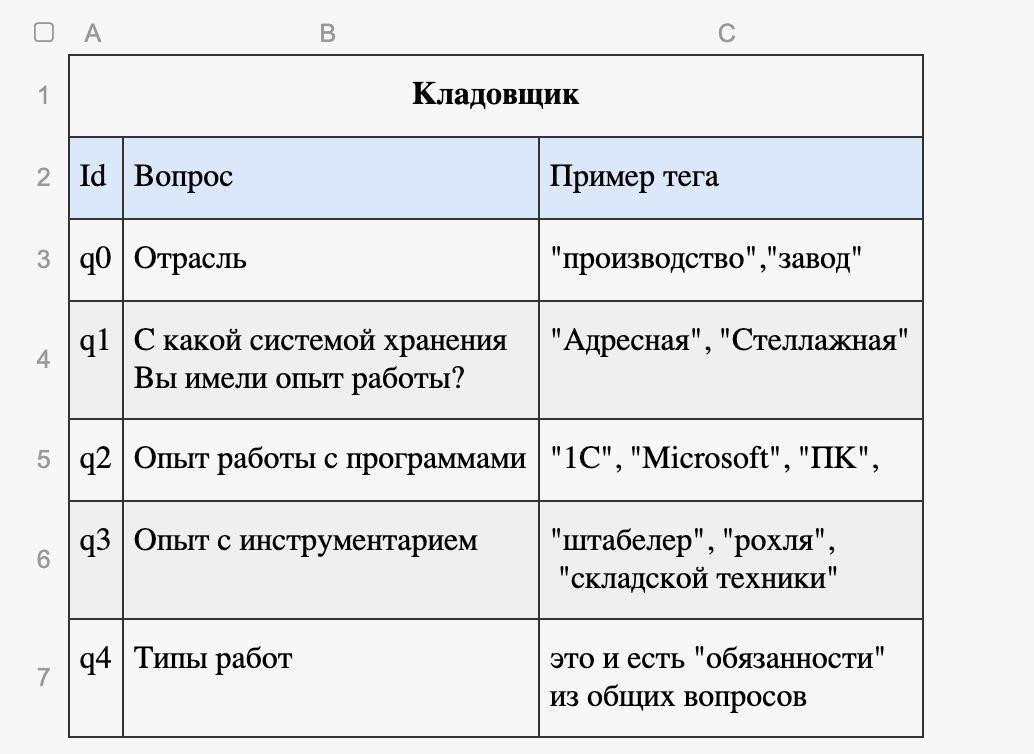
\includegraphics[width=8cm]{"./images/sample.jpg"}
		\centering
	\end{figure}
\end{frame}


\begin{frame}
	\frametitle{Результат работы алгоритма}

	\begin{figure}[t]
		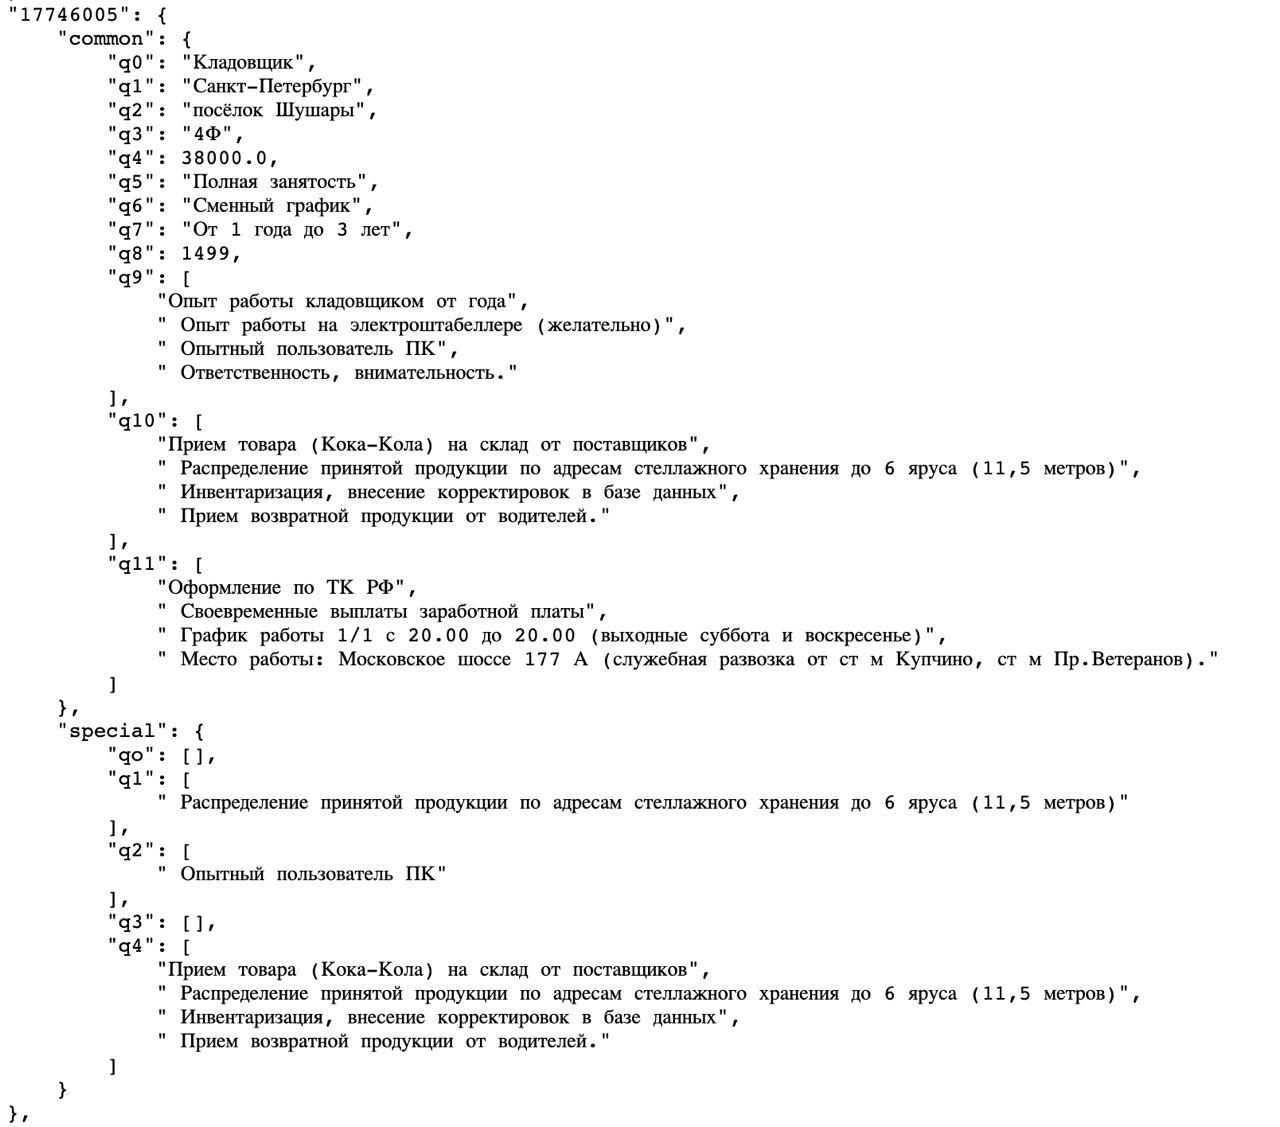
\includegraphics[width=8cm]{"./images/result.jpg"}
		\centering
	\end{figure}
\end{frame}


\begin{frame}
	\frametitle{Преимущества}

	\begin{itemize}
		\item Решение полностью работает для таблицы вакансий
		\item Оно масшабируемое
		\item Быстро работает
        \item Не требовательно к вычислительным ресурсам
		\item Теги уже есть на многих сайтах по поиску работы
	\end{itemize}
\end{frame}


\begin{frame}
	\frametitle{Что можно добавить}

	\begin{itemize}
		\item Искать включения без тегов по расстоянию между вопросом и смысловой единицей
		\item Выводить вопросы, на которые не были получены ответы
	\end{itemize}
\end{frame}


\begin{frame}
	\frametitle{Контакты}

	\begin{itemize}
        \item @taya\_penskaya
        \item @furiousteabag
        \item @Libkneht
	\end{itemize}
\end{frame}



\end{document}
